\subsection{Evaluation Function}
\label{sec:evaluation_function}

This section describes the static evaluation function used by the engine. Since
the search explores only a limited portion of the game tree, a heuristic
evaluation is required to estimate the quality of non-terminal positions. The
implemented evaluation follows a classical \emph{tapered} approach with separate
midgame (MG) and endgame (EG) scores, piece-square tables (PSQT), a phase-based
interpolation scheme, and a tempo bonus.

\subsubsection{Material Model}
\label{subsec:material_model}

The evaluation assigns a material value to each piece type. Material is counted
for both sides and is added to the positional contribution of the corresponding
piece-square table. Conceptually, for a piece on square $s$, the score is:
\[
\text{score}(p,s) = \text{material}(p) + \text{psqt}(p,s).
\]
In the implementation, material values are used in two variants: a midgame value
and an endgame value. This is consistent with the idea that the relative
importance of pieces changes over the course of a game (e.g., kings become more
active in endgames).

\subsubsection{Piece-Square Tables (PSQT)}
\label{subsec:psqt}

Positional preferences are encoded using piece-square tables. For each piece
type, the engine stores a 64-entry table for midgame and endgame, assigning a
positional bonus (or penalty) to each square. This model captures common chess
principles such as centralization, piece activity, and king safety without
explicit feature engineering.

The implementation uses a single table orientation and mirrors squares for the
white pieces by applying a rank flip. Concretely, for a board index $i$,
white pieces use index $i \oplus 56$, while black pieces use $i$ directly. This
ensures that both colours share the same PSQT semantics relative to their
respective perspective.

\subsubsection{Midgame and Endgame Separation}
\label{subsec:mg_eg}

Instead of a single score, the evaluation computes two scores:
\begin{itemize}
    \item $MG$: midgame score (material + PSQT using MG tables),
    \item $EG$: endgame score (material + PSQT using EG tables).
\end{itemize}

The engine accumulates these values separately for both sides. The final score
is then expressed from the perspective of the \emph{side to move}. This is
implemented by subtracting the opponent's accumulated values from the values of
the player whose turn it is.

\subsubsection{Game Phase Interpolation}
\label{subsec:phase_interpolation}

To smoothly transition between midgame and endgame behavior, the engine uses a
tapered evaluation. A game-phase value is computed as the sum of per-piece phase
contributions. The resulting phase is clamped to a maximum of $24$, yielding:
\[
mgPhase = \min(24, \text{phase}(P)), \qquad egPhase = 24 - mgPhase.
\]
The final evaluation is obtained by linear interpolation:
\[
Eval(P) = \frac{MG(P)\cdot mgPhase + EG(P)\cdot egPhase}{24}.
\]
This approach is commonly used in classical engines, as it avoids abrupt
evaluation changes and provides a simple, interpretable blending scheme.

\begin{figure}[ht]
\centering
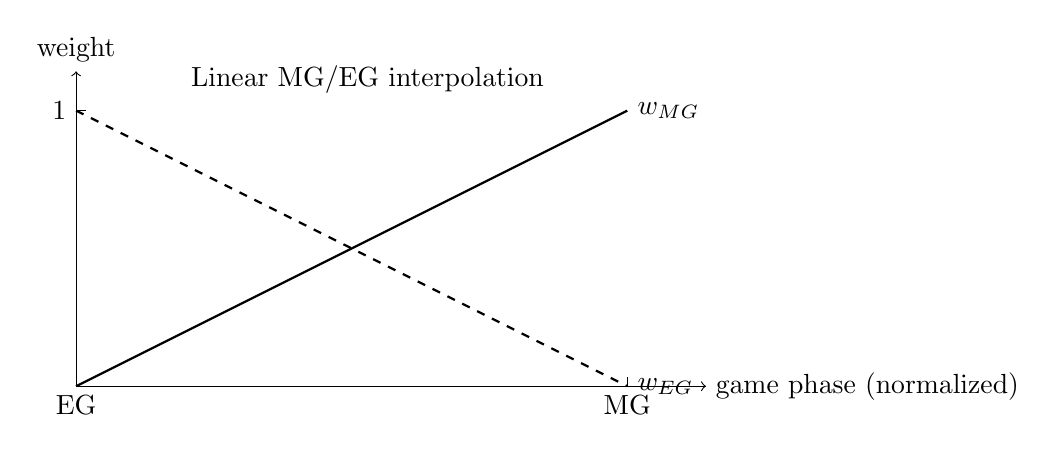
\begin{tikzpicture}[scale=1.0]
  \draw[->] (0,0) -- (8,0) node[right] {game phase (normalized)};
  \draw[->] (0,0) -- (0,4) node[above] {weight};

  % mg weight line: 0..1
  \draw[thick] (0,0) -- (7,3.5) node[right] {$w_{MG}$};
  % eg weight line: 1..0
  \draw[thick,dashed] (0,3.5) -- (7,0) node[right] {$w_{EG}$};

  % ticks
  \foreach \x/\lab in {0/EG,7/MG}{
    \draw (\x,0) -- (\x,0.12);
    \node[below] at (\x,0) {\lab};
  }
  \draw (0,3.5) -- (0.12,3.5);
  \node[left] at (0,3.5) {1};

  \node at (3.7,3.9) {Linear MG/EG interpolation};
\end{tikzpicture}
\caption{Tapered evaluation: midgame and endgame weights vary linearly with the
game phase.}
\label{fig:tapered_eval}
\end{figure}

\subsubsection{Tempo Bonus}
\label{subsec:tempo_bonus}

A constant tempo bonus is added to the final score to reflect the advantage of
having the next move. In the implementation, the returned evaluation is:
\[
Eval_\text{final}(P) = Eval(P) + 20.
\]
Since the engine evaluates positions from the perspective of the side to move,
this constant shifts the score slightly in favor of the player whose turn it is,
encouraging initiative and reducing symmetry artifacts.

\subsubsection{Algorithmic Summary}
\label{subsec:eval_algorithm}

\begin{algorithm}[ht]
\DontPrintSemicolon
\KwIn{Board position $P$}
\KwOut{Static evaluation score from the perspective of the side to move}

Initialize $mg[2]\gets 0$, $eg[2]\gets 0$, $phase\gets 0$\;

\For{$i \gets 0$ \KwTo $63$}{
    $piece \gets P[i]$\;
    $phase \gets phase + phaseValue(piece)$\;
    \uIf{$piece$ is white}{
        $idx \gets i \oplus 56$\tcp*{mirror for white}
        $mg[W] \gets mg[W] + MG\_PSQT(piece, idx) + MG\_MAT(piece)$\;
        $eg[W] \gets eg[W] + EG\_PSQT(piece, idx) + EG\_MAT(piece)$\;
    }
    \uElseIf{$piece$ is black}{
        $idx \gets i$\;
        $mg[B] \gets mg[B] + MG\_PSQT(piece, idx) + MG\_MAT(piece)$\;
        $eg[B] \gets eg[B] + EG\_PSQT(piece, idx) + EG\_MAT(piece)$\;
    }
}

$mgPhase \gets \min(24, phase)$\;
$egPhase \gets 24 - mgPhase$\;

Compute $MG(P)$ and $EG(P)$ as difference between side-to-move and opponent\;
$Eval(P) \gets \big(MG(P)\cdot mgPhase + EG(P)\cdot egPhase\big) / 24$\;

\Return $Eval(P) + 20$\tcp*{tempo}
\caption{Static evaluation with MG/EG separation, tapered interpolation, and tempo bonus.}
\label{algo:evaluation}
\end{algorithm}

\subsubsection{Limitations of the Evaluation}
\label{subsec:eval_limitations}

The evaluation is intentionally simple and focuses on material and PSQT-based
positional features. This makes it fast and easy to analyze, but it also implies
several limitations:
\begin{itemize}
    \item \textbf{Limited feature set:} Pawn structure (isolated/doubled/passed
    pawns), mobility, rook activity on open files, bishop pair, and advanced king
    safety concepts are not modeled explicitly.
    \item \textbf{No explicit drawishness detection:} The evaluation does not
    implement specialized scaling for fortress-like positions, opposite-coloured
    bishop endgames, or other draw-prone material configurations.
    \item \textbf{Constant tempo term:} The tempo bonus is a fixed constant and
    does not depend on phase or position characteristics.
    \item \textbf{No incremental evaluation:} The score is computed by scanning
    all 64 squares, rather than updating evaluation terms incrementally during
    make/unmake.
\end{itemize}

Despite these limitations, the evaluation is sufficient for the primary focus of
this thesis, namely the investigation of search behavior and iterative deepening
under time constraints. A stronger evaluation can be integrated later without
changing the surrounding search architecture.